\documentclass[12pt]{article}
\usepackage[utf8]{inputenc}
\usepackage[english]{babel}
%\usepackage{amsmath}
%\usepackage{amsfonts}
%\usepackage{amssymb}
%\usepackage{amsmath}
%\usepackage{amsthm}
%\usepackage{latexsym}
%\usepackage{amscd}
\usepackage{graphics}
\usepackage{graphicx}
\usepackage[pdftex,linktocpage=true,bookmarks=true,bookmarksnumbered=true,colorlinks,linkcolor=blue,citecolor=red]{hyperref}
%\usepackage{anysize}
%\usepackage{epstopdf}
%\usepackage{pst-all}
%\usepackage{pstricks}
%\usepackage{url}
%\usepackage{float}
%\usepackage[T1]{fontenc}
%\usepackage{textcomp}
%\usepackage{color}

%%%%%%%%%%%%%%%%%%%%%%

%opening
\title{A model of packages moving through a network.}
\author{J. Villalobos}

\date{\today}

%%%%%%%%%%%%%%%%%%%%%%

\begin{document}

\maketitle

\begin{abstract}
  \textcolor{red}{\large {\bf FALTA}}
\end{abstract}


%%%%%%%%%%%%%%%%%%%%%%%%%%%%%%%
%\section{Introduction}
%%%%%%%%%%%%%%%%%%%%%%%%%%%%%%%

%%%%%%%%%%%%%%%%%%%%%%%%%%%%%%%
\section{The Model}
%%%%%%%%%%%%%%%%%%%%%%%%%%%%%%%

We simulate traffic on a network using the following setup:
\begin{itemize}
  \item Time is discrete. The unit is a tick; we represent it by $t$.
  \item A graph represents the network; we use $M$ for the number of nodes.
  \item We use packages to represent traffic that may move between nodes each tick. 
  \item There are $P$ packages within the network at any given tick. $P$ is kept constant through a simulation.
  \item We use $K$ for the maximum number of packages that a node may hold. 
    Therefore, each node $m \in [0,1,\ldots,M]$ has a number of packages $0 \le p_m(t) \le K$ at a given time.    
  \item Since the total number of packages is kept constant through the simulation, we have that $\sum_{m=1}^M p_m(t) = P$, for all $t$.
  \item Individual nodes operate under the following rules:
  \begin{itemize}
    \item Each has a fixed capacity of $K$ (the maximum number of packages that can occupy a node at a given tick).
    \item Each tick, every node chooses a neighbor node at random and tries to send a package to it.
    \item Each tick a node may receive any number of packages between 0 and its in-degree.
    \item If the number of received packages plus the actual number of packages is larger than $K$, no packages are accepted (they are all returned to the neighbors that sent the packages).
  \end{itemize}
  \item Each edge has one of two states: open (green) or closed (red).
  \begin{itemize}
    \item Open means that a package may travel between the nodes connected by the edge; closed means that it may not.
    \item The state of edges changes with time based on two parameters: $\omega_{j,k} \ge 0$ and $\phi_{j,k} \in [0, 2 \pi]$.
      The subscripts $j$, $k$ indicate that the edge connects node $j$ with node $k$.
    \item An edge that connects node $j$ to node $k$ is open at time $t$ if $\sin(\omega_{j,k} t + \phi_{j,k}) \ge 0$.
    \item An edge that connects node $j$ to node $k$ is closed at time $t$ if $\sin(\omega_{j,k} t + \phi_{j,k}) < 0$.
  \end{itemize}
\end{itemize}



%%%%%%%%%%%%%%%%%%%%%%%%%%%%%%%
\section{Some experiments}
%%%%%%%%%%%%%%%%%%%%%%%%%%%%%%%

We will use four different networks on which to run simulations.
A set of connections defines a graph.
We use the notation $u \leftrightarrow v$ to denote a two-way or undirected link between node $u$ and $v$ (a single arrow indicates a directed link).
The definitions of the four networks are:
\begin{enumerate}
  \item A complete network is one on which all possible connections are available.
    This is $\{u \leftrightarrow v\}$, $\forall u \neq v$.
  \item A circle network in one on which every node has two connections.
    The graph is defined by: $\{1  \leftrightarrow 2, 2 \leftrightarrow 3, 3 \leftrightarrow 4, \dots m \leftrightarrow m+1, \ldots, M-1 \leftrightarrow M, M \leftrightarrow 1\}$.
  \item A square grid, a network in which every node has four neighbors, except for four nodes (corners) with precisely two neighbors, and some nodes (the edges) that have three neighbours each; we will only use square grids.
    This means that $M$ will always be an integer square.
  \item A Barabasi-Albert graph, constructed starting from a circular graph of three nodes, subsequently add a vertex with two edges at each step. The edges are attached to vertices at random, following a distribution proportional to the vertex degree.
\end{enumerate}

We propose two different setups for simulations: keeping the edges open at all time and opening and closing the edges according to fixed values of $\omega_{j,k} \ge 0$ and $\phi_{j,k}$.
We start running simulations on undirected networks and follow with directed networks.

\subsection{Undirected Networks}
\label{sec:undirected}

We build average flow, $\bar{J}$, versus density, $\rho$, plots.
The average flow is the mean number of packages that moved on an ensemble of simulations (we run 40 simulations of 300 ticks each). 
We normalize the flow to the number of nodes on the network.
The density $\rho$ is the number of packages in the network divided by the product of the number of nodes and the capacity of the nodes; this is $\rho = \frac{P}{M \times K}$.

On an undirected network, if a package can travel from node $a$ to node $b$, then it can always do it from $b$ to $a$.


\subsubsection{All links open}
\label{sec:undirected-open}

We start by running simulations on undirected networks of $M=100$ nodes, with open edges.
All simulations are carried out 

With all the links open all the time we get that $\bar{J}$ behaves as depicted in Fig. \ref{fig:JvsrhoAllOpen}
We see that for the four types of networks, and different values of $K$ (2, 5, 10, and 100) the average flow $\bar{J}$ starts at 0, for $\rho=0$ and grows as $\rho$ gets bigger, then it comes to a plateau and starts decreasing in an almost symetric way.
The height of the maximum depends on the value of $K$ and is slightly shifted depending of the type of network.

\begin{figure}[!hbt]
  \centering
  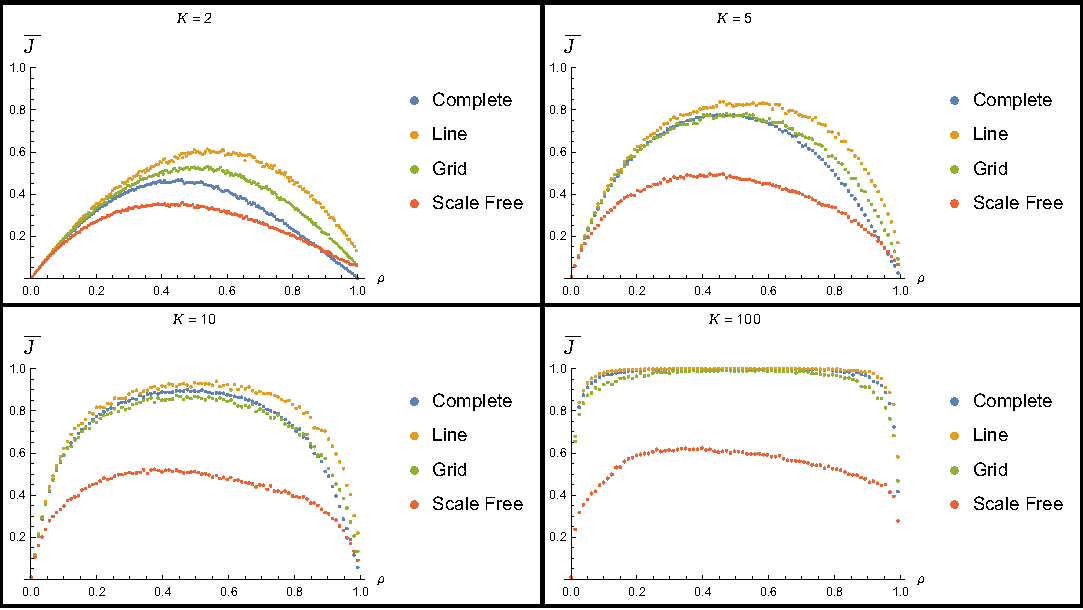
\includegraphics[width=\textwidth]{plots/fundamentalUndirected.pdf}
  \caption{Average flow $\bar{J}$ Vs. density $\rho$ for four types of networks.}
  \label{fig:JvsrhoAllOpen}
\end{figure}

It is expected that the flow is 0 for both $\rho = 0$ and $\rho =1$ since in the first case we have $m=0$ (no packages in the network), and for $\rho = 1$ we have $m = M K$, which means that all nodes have $K$ packages (no movement is possible in this situation).
The flow behaves differently for the scale-free network, it is always inferior to the other networks. 
This is also expected given that the degree distribution of such network is different from the other ones: the degree distribution is uniform for the complete and circle network, and it is almost uniform for the grid (all nodes on the grid have four neighbours, except for the four corners that have 2 neighbours).
On a scale-free network there are few nodes with lots of neighbours, while most modes have a small degree, the nodes with a high degree fill up with packages and hinder flow.
Note that this is the case even for high values of $K$

\begin{figure}[!hbt]
  \centering
  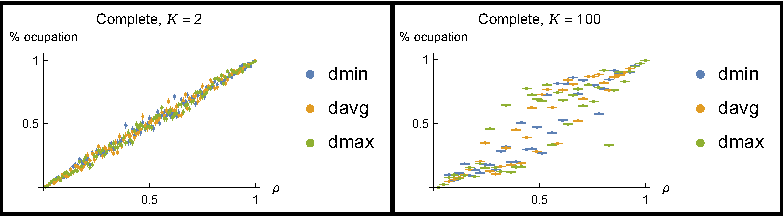
\includegraphics[width=\textwidth]{plots/ocupationVarianceComplet.pdf}
  \caption{Ocupation percentage Vs. density $\rho$ for the coplete network for $K=2$ (left), and $k=100$ (right). 
    The ocupation is shown for three nodes: dmin, dmax and davg (see text for the definitions).}
  \label{fig:perOcComplete}
\end{figure}

Figures \ref{fig:perOcComplete} through \ref{fig:perOcScaleFree} show the ocupation percentage Vs. $\rho$ for the different networks and different values of $K$.
We use one simulation of 300 ticks for 40 different values of $\rho$.
The ocupation percentage is the mean number of packages at a given node, divided by $K$ (the capacity of the node); we calculate this percentage as the mean of the packages that are on the node on a given simulation, we plot this mean with bars that mark standard deviation normalized to the number of ticks used on the simulation.
Each plot shows the behavior of a different node picked randomly based on the following definitions: dmin reffers to a node that has the minimum degree in the network, dmax is a node that has the maximum degree of the network and davg is a node, as close as possible, to the floor of the average degree of the network.

Figure \ref{fig:perOcComplete} shows the ocupation percentage for the complete network. 
Since on this networks all the nodes have the same degree (the number of nodes minus one), we have that dmin, dmax, and davg are any node.
The subplot on the left was made with maximum ocupation $K=2$, the one on the right with $K=100$.
As expected, when there are no packagen in the network ($\rho =0$), the occupation is 0, and when the number of packages is $K$ in every node ($\rho=1$) the occupation is 1.
When the maximum occupation number is small ($K=2$), the occupation correlates linearly with the density of packages, we can say it is uniform through the network; this is expected since there can't be much flow due to the restriction in the number of packages per node.
When the maximum occupation number is large ($K=100$), the occupation behaves erraticly and all three nodes behave differently; unless $\rho$ is close to 0 or to 1, the occupation on each node is different from the one in another.
This is due to the fact that all nodes are equal in this particular network.

\begin{figure}[!hbt]
  \centering
  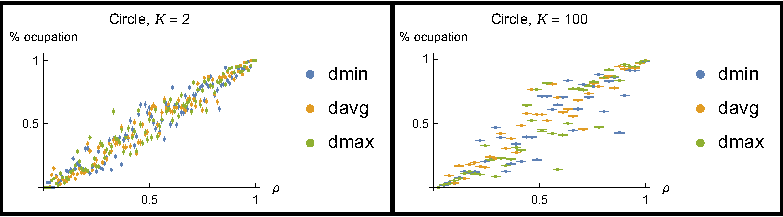
\includegraphics[width=\textwidth]{plots/ocupationVarianceCircle.pdf}
  \caption{Ocupation percentage Vs. density $\rho$ for the circle network for $K=2$ (left), and $k=100$ (right). 
    The ocupation is shown for three nodes: dmin, dmax and davg (see text for the definitions).}
  \label{fig:perOcCircle}
\end{figure}

Figure \ref{fig:perOcCircle} shows the ocupation percentage for the circle network. 
Since on this networks all the nodes have the same degree (they all have two neighbours), we have that dmin, dmax, and davg are any node.
The subplot on the left was made with maximum ocupation $K=2$, the one on the right with $K=100$.
Given that this network is similar to the complete one (all nodes have the same degree), the observed behaviour is very similar. 
When the maximum occupation number is small ($K=2$), the occupation correlates linearly with the density of packages, we can say it is uniform through the network; this is expected since there can't be much flow due to the restriction in the number of packages per node added to the restriction that there are few nodes that may recieve pakages.
When the maximum occupation number is large ($K=100$), the occupation behaves erraticly and all three nodes behave differently; unless $\rho$ is close to 0 or to 1, the occupation on each node is different from the one in another.
As with the complete network, this is due to the fact that all nodes are equal in this particular network.



\subsubsection{Links changing states}
\label{sec:undirected-red-green}


	
\subsection{Directed Networks}
\label{sec:directed}

Under construction

\end{document}